\documentclass{beamer}
\usetheme[nat]{Frederiksberg}

\usepackage{algorithm}
\usepackage[noend]{algorithmic}
\usepackage{adjustbox}
\usepackage{multirow}
\usepackage{siunitx}
\usepackage{amsmath}

\begin{document}
\title{Master's thesis defense}
\author{Nikolaj Dybdahl Rathcke}
\date{June 27, 2018}

\frame{\titlepage}

% New page

\section{Motivation and Problem Definition}
\frame{\frametitle{Motivation and Problem Definition}
\begin{columns}[c]
  \column[b]{6cm}
  \begin{itemize}
    \item The \textit{distance oracle}.
    \item Performance measures
    \item The vertex-labeled variant.
  \end{itemize}
  \column{4cm}
  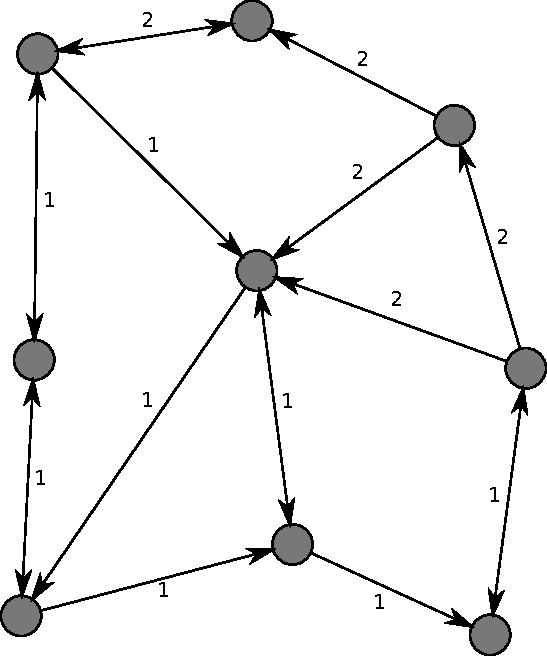
\includegraphics[width=\textwidth]{figs/intro.pdf}
\end{columns}

}

% New page

\section{Motivation and Problem Definition}
\frame{\frametitle{Motivation and Problem Definition}
\begin{columns}
  \column{6cm}
  \textbf{The distance oracle}. \\
  $ $ \\
  A compact data structure that can quickly answer shortest paths between two vertices $u$ and
  $v$.
  \column{4cm}
  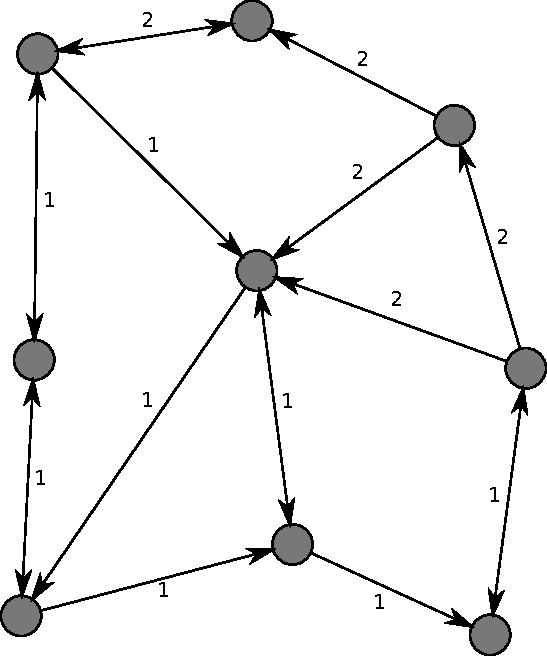
\includegraphics[width=\textwidth]{figs/intro.pdf}
\end{columns}

}

% New page

\section{Motivation and Problem Definition}
\frame{\frametitle{Motivation and Problem Definition}
\begin{columns}[c]
  \column{6cm}
  \textbf{Performance measures}. \\
  $ $ \\
  \textit{Space}. The size of the data structure. \\
  $ $ \\
  \textit{Query time}. The time it takes to answer shortest path queries. \\
  $ $ \\
  \textit{Preprocessing time}. The time it takes to build the data structure. \\
  $ $ \\
  \textit{Update time}. Time it takes to adjust the data structure
  to reflect changes to the graph.
  \column{4cm}
  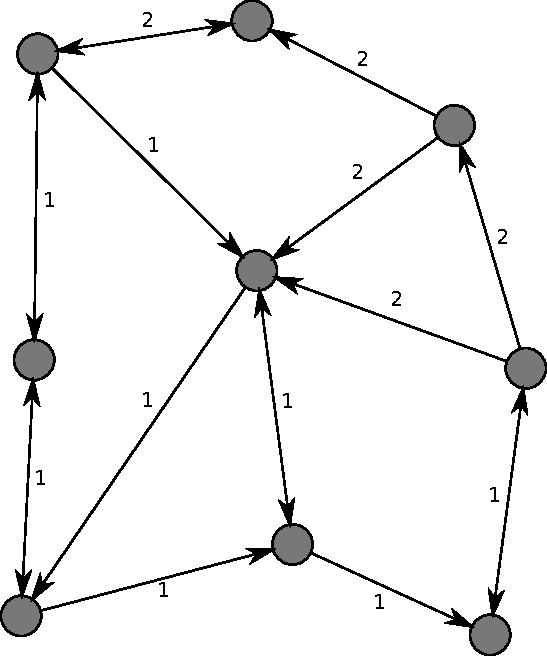
\includegraphics[width=\textwidth]{figs/intro.pdf}
\end{columns}

}

% New page

\section{Motivation and Problem Definition}
\frame{\frametitle{Motivation and Problem Definition}
\begin{columns}[c]
  \column{6cm}
  \textbf{The vertex-labeled variant}. \\
  $ $ \\
  Each vertex is associated with a label $\lambda$ from a set of labels $L=\{\lambda_1,
  \dots, \lambda_\ell\}$. \\
  Instead of answering shortest path between two vertices, we answer shortest path
  queries,  $Q(u,\lambda)$, from a vertex $u$ to the nearest $\lambda$-labeled vertex.
  \column{4cm}
  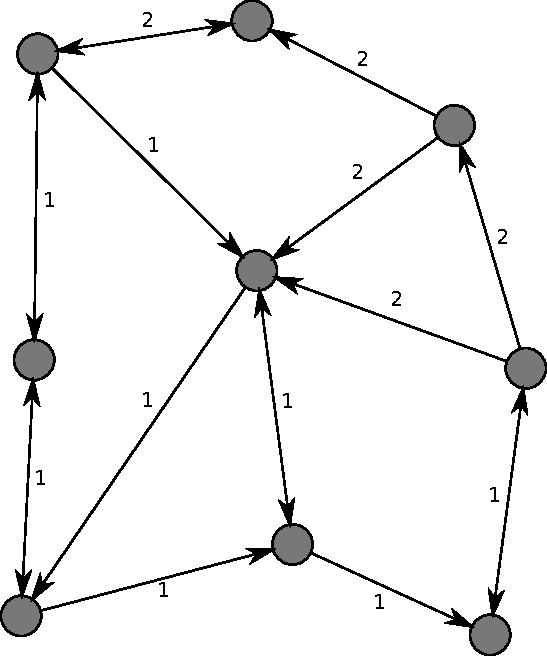
\includegraphics[width=\textwidth]{figs/intro.pdf}
\end{columns}

}

% New page

\section{Motivation and Problem Definition}
\frame{\frametitle{Motivation and Problem Definition}
\begin{columns}[c]
  \column{6cm}
  \begin{itemize}
    \item The \textit{distance oracle}.
    \item Performance measures
    \item The vertex-labeled variant.
  \end{itemize}
  \noindent $ $\\
  \textbf{This thesis}: Distance oracles in directed planar vertex-labeled graphs.
  \column{4cm}
  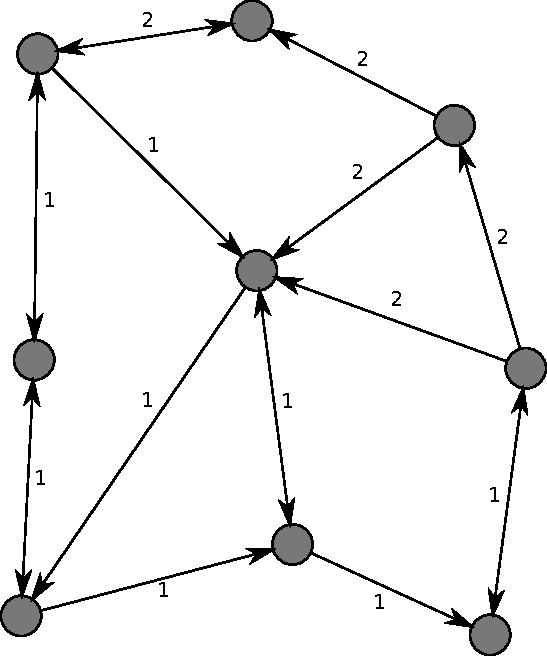
\includegraphics[width=\textwidth]{figs/intro.pdf}
\end{columns}

}

% New page

\section{Results}
\frame{\frametitle{Results}

  \begin{block}{Theorem 1}
    \small
    There is a distance oracle with space $O(n\ell^{2/3})$, query time $O(\ell^{1/3})$
    and preprocessing time $\tilde{O}(n\ell^{2/3})$.
  \end{block}
  \begin{block}{Theorem 2}
    \small
    There is a distance oracle that can handle edge-weight changes, edge insertions and
    deletion in amortized $O(n^{2/3}\lg^{5/3} n)$ time. It can be constructed using
    $O(n\lg n)$ space in $O(n\lg n)$ time, and answers queries in
    $\tilde{O}(\min\{\text{size}(\lambda)\cdot n^{2/3}, n\})$ time.
  \end{block}
  \begin{block}{Theorem 3}
    \small
    Under the assumption that $G$ does not have $\omega(\sqrt{n})$ labels of polynomial
    size, there is a distance oracle with space $O(n^{3/2})$, query time
    $O(\text{polylog}(n))$ and preprocessing time $\tilde{O}(n^{3/2})$. Furthermore, it
    can handle labels changes in expected $O(1)$ time.
  \end{block}

}

% New page |||||| First oracle

\section{Warm-up: An oracle depending on $\ell$}
\frame{\frametitle{Warm-up: An oracle depending on $\ell$}

  \begin{block}{Theorem 1}
    \small
    There is a distance oracle with space $O(n\ell^{2/3})$, query time $O(\ell^{1/3})$
    and preprocessing time $\tilde{O}(n\ell^{2/3})$.
  \end{block}

\begin{columns}[c]
  \column{10cm}
  \begin{itemize}
    \item Built on top of an $r$-division.
    \item Store shortest paths to all labels from \textit{boundary vertices}.
    \item Store shortest paths from all \textit{interior vertices} to all labels in the
      same piece and to all boundary vertices of the piece.
  \end{itemize}
\end{columns}

}

% New page

\section{The $r$-division}
\frame{\frametitle{The $r$-division}

  Given some $r$, an $r$-division is a collection of connected subgraphs that satisfy:
  \begin{itemize}
      \item Any edge belongs to one region.
      \item There are $O(n/r)$ regions.
      \item For each region, there are $O(\sqrt{r})$ boundary vertices.
      \item For each region, there are $O(r)$ vertices.
  \end{itemize}
  \begin{center}
  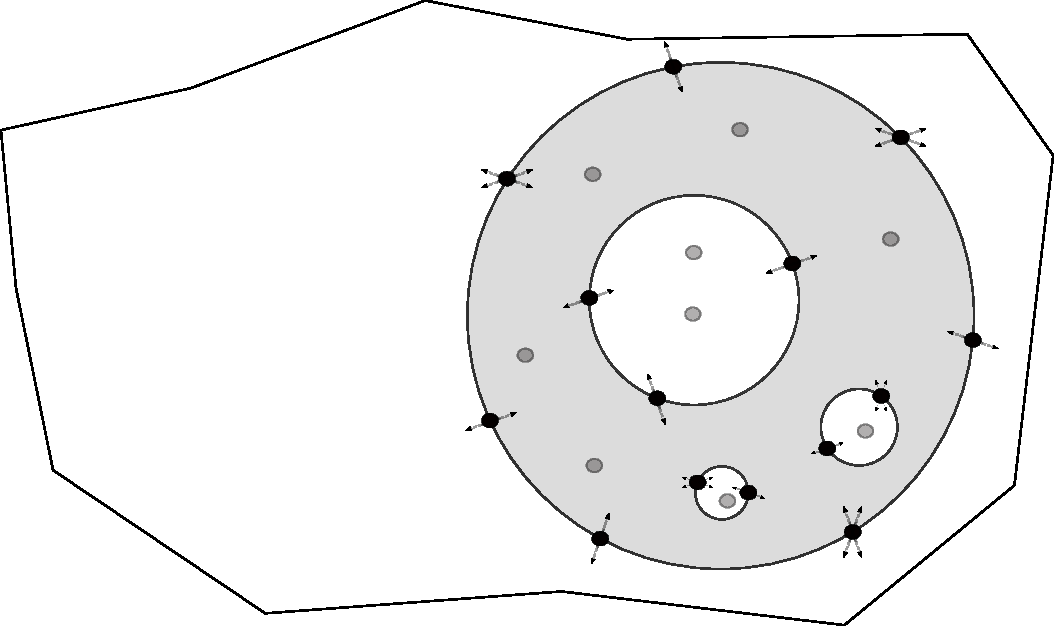
\includegraphics[scale=0.33]{figs/rdiv.pdf}
\end{center}

}

% New page

\section{The $r$-division}
\frame{\frametitle{The $r$-division}

  Given some $r$, an $r$-division is a collection of connected subgraphs that satisfy:
  \begin{itemize}
      \item Any edge belongs to one region.
      \item There are $O(n/r)$ regions.
      \item For each region, there are $O(\sqrt{r})$ boundary vertices.
      \item For each region, there are $O(r)$ vertices.
  \end{itemize}
  There is version due to Klein, Sommer and Mozes giving a decomposition tree that further guarantees:
  \begin{itemize}
    \item Each piece $O(1)$ holes.
    \item On any level of the decomposition, we have $O(\sqrt{n})$ boundary vertices in
      total.
    \item Can be computed in $O(n)$ time.
  \end{itemize}

}

% New page

\section{The oracle}
\frame{\frametitle{The oracle}
  We store the following:
  \begin{itemize}
    \item Store shortest path from boundary vertices to all labels outside a region.
    \item Store shortest path from all interior vertices to all boundary vertices of the
      region as well as all labels inside the same
      region.
  \end{itemize}
  \begin{center}
  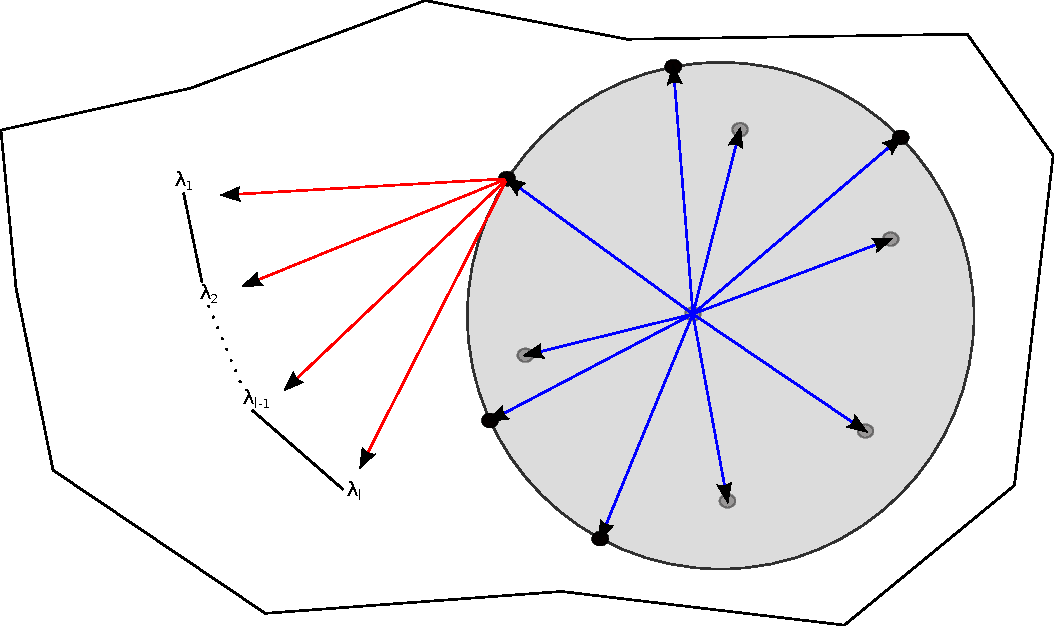
\includegraphics[scale=0.4]{figs/oracle1.pdf}
\end{center}

}

% New page

\section{The oracle}
\frame{\frametitle{The oracle}
  Given the query $Q(u,\lambda)$, find all distances $\delta(u,b)+\delta(b,\lambda)$ and
  the distance $\delta(u,\lambda)$ stored for $u$ inside the region. Return the minimum.
  \begin{center}
    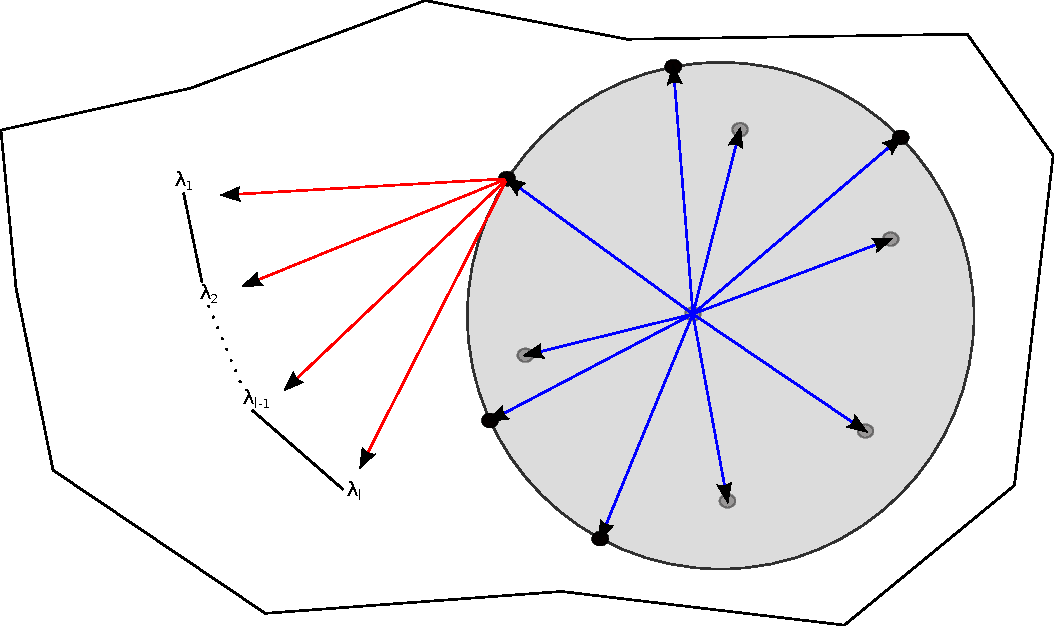
\includegraphics[scale=0.4]{figs/oracle1.pdf}
  \end{center}

}

% New page

\section{The oracle}
\frame{\frametitle{The oracle: Analysis}

  \textbf{Query}. Bounded by the number of boundary vertices, which is $O(\sqrt{r})$ \\
  $ $ \\
  \textbf{Space}. We have $O(n/r)$ regions, so $O(n/\sqrt{r})$ boundary vertices. For any
  interior vertex, we store up to $O(r)$ distances, yielding $O(n\ell/\sqrt{r}+nr)$
  space. \\
  $ $ \\
  \textbf{Preprocessing}. Compute SSSP from boundary vertices in $O(n)$ time. We then
  know distances between boundary vertices, so we can compute interior distances using
  Djikstra in $O(r\lg r)$ time. This gives us $O(n^2/\sqrt{r}+nr\lg r)$ preprocessing.

}

% New page

\section{The oracle}
\frame{\frametitle{The oracle: Analysis}

  \textbf{Query}: $O(\sqrt{r})$ \\
  \textbf{Space}: $O(n\ell/\sqrt{r}+nr)$ \\
  \textbf{Preprocessing}: $O(n^2/\sqrt{r}+nr\lg r)$ \\
  $ $ \\
  Pick $r=\ell^{2/3}$ to get Theorem 1:

  \begin{block}{Theorem 1}
    \small
    There is a distance oracle with space $O(n\ell^{2/3})$, query time $O(\ell^{1/3})$
    and preprocessing time $\tilde{O}(n\ell^{2/3})$.
  \end{block}

}

% New page |||||| Second oracle

\section{A dynamic vertex-labeled distance oracle}
\frame{\frametitle{A dynamic vertex-labeled distance oracle}

  \begin{block}{Theorem 2}
    \small
    There is a distance oracle that can handle edge-weight changes, edge insertions and
    deletion in amortized $O(n^{2/3}\lg^{5/3} n)$ time. It can be constructed using
    $O(n\lg n)$ space in $O(n\lg n)$ time, and answers queries in
    $\tilde{O}(\min\{\text{size}(\lambda)\cdot n^{2/3}, n\})$ time.
  \end{block}

\begin{columns}[c]
  \column{10cm}
  \begin{itemize}
    \item Built on an $r$-division.
    \item FR-Djikstra variant.
      \begin{itemize}
        \item Dense distance graph.
        \item Fast query using Djikstra and exploiting the Monge property in the DDG.
      \end{itemize}
    \item Henzinger's SSSP algorithm to avoid terrible worst-case times.
  \end{itemize}
\end{columns}

}

% New page

\section{FR-Djikstra}
\frame{\frametitle{The Dense Distance Graph}

  The dense distance graph (DDG) is the graph where there is an edge between
  boundary vertices of the same piece $P$ with weight equal to the shortest path in $P$.

}

% New page

\section{The oracle}
\frame{\frametitle{The oracle}

  TODO

}

% New page |||||| Third oracle

\section{An oracle with better query times}
\frame{\frametitle{An oracle with better query times}

  \begin{block}{Theorem 3}
    \small
    Under the assumption that $G$ does not have $\omega(\sqrt{n})$ labels of polynomial
    size, there is a distance oracle with space $O(n^{3/2})$, query time
    $O(\text{polylog}(n))$ and preprocessing time $\tilde{O}(n^{3/2})$. Furthermore, it
    can handle label changes in expected $O(1)$ time.
  \end{block}

\begin{columns}[c]
  \column{10cm}
  \begin{itemize}
    \item Built on top of an $r$-division.
    \item Store all shortest paths to and from boundary vertices.
    \item Store \textit{additiviely weighted Voronoi diagrams} for all vertices $u$ and
      a constant number of holes $h$.
    \item Point to point distances in $O(\lg n)$ time using weighted Voronoi diagrams.
    \item Hash tables to keep track of what vertices have what labels.
  \end{itemize}
\end{columns}

}

% New page

\section{Additively weighted Voronoi diagrams}
\frame{\frametitle{Additively weighted Voronoi diagrams}

  dksa \\
  dskjadjs \\
  dsakda \\
  \centering
  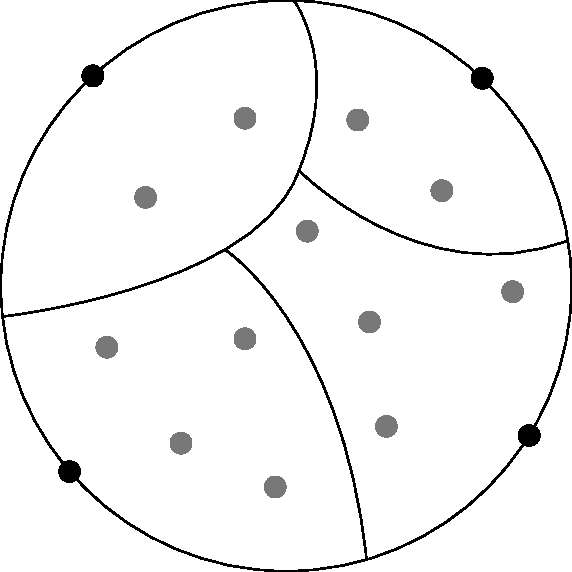
\includegraphics[scale=0.3]{figs/awvd1.pdf}
  \ \ \
  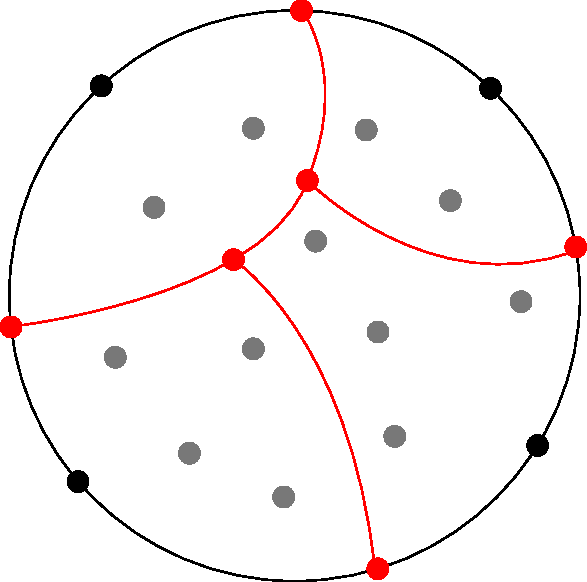
\includegraphics[scale=0.3]{figs/awvd2.pdf}


}

% New page

\section{Conclusion and future work}
\frame{\frametitle{Conclusion and future work}

  TODO

}



\end{document}
